\documentclass[10pt, journal,onecolumn]{IEEEtran}
\usepackage{cite}
\usepackage{graphicx}
\graphicspath{{figure/}}
\usepackage{array}
\usepackage{subfigure}
\usepackage{stfloats}
\usepackage{url}
\usepackage{nicefrac}
\usepackage{amssymb}
\usepackage{amsmath}
\usepackage{amsfonts}
\usepackage{amssymb}
\usepackage{booktabs}
\usepackage{relsize}
\usepackage[pdfpagelabels]{hyperref}
\usepackage{float}
\usepackage[round]{natbib}
\usepackage{color}
\usepackage{authblk}
\usepackage{caption}
\usepackage{enumerate}

\newcommand{\ra}[1]{\renewcommand{\arraystretch}{#1}}

\hypersetup{
  colorlinks   = true, %Colours links instead of ugly boxes
  urlcolor     = blue, %Colour for external hyperlinks
  linkcolor    = red, %Colour of internal links
  citecolor   = red %Colour of citations
}

\floatstyle{ruled}
\newfloat{algorithm}{tbp}{loa}
\floatname{algorithm}{Algorithm}

\newtheorem{theorem}{Theorem}
\newtheorem{corollary}{Corollary}
\newtheorem{proposition}{Proposition}
\newtheorem{definition}{Definition}
\newtheorem{lemma}{Lemma}

\newcommand{\norm}[1]{\left\lVert#1\right\rVert}
\newcommand{\abs}[1]{\left\lvert#1\right\rvert}
\newcommand{\inner}[1]{\left\langle#1\right\rangle}
\def\b#1{\mathbf{#1}}
\def\t#1{\text{#1}}


\title{Predicting the 2014 Ebola Outbreak in West Africa using Network Analysis \\
       {\large Final Report} }

\author{Shafi Bashar, Mike Percy, Romit  Singhai}
\affil{\textit {\{shafiab, mp81, romit\}@stanford.edu}}

\renewcommand\Authands{ and }

\begin{document}

\maketitle


%I%%%%%%%%%%%%%%%% INTRODUCTION %%%%%%%%%%%%%%%%%%%%%%

\section{{Introduction and Motivation}}
\label{sec:Introduction}

The 2014 Ebola epidemic in the West African nations of Guinea, Sierra Leone and Liberia is the
largest in history. As of writing this report, more than 17,000
suspected cases have been reported by the WHO (World Health Organization) and the numbers continue
to rise. In this project, we explore
the time-series data available for the current Ebola epidemic and perform analysis, model-fitting and
short-term forecasting of epidemic spread at the local (country) level as well as at a world-wide scale by
using economic trade network, geographical, and population data in concert with network and epidemiological theory.

Traditional epidemiological analysis is typically based on subdividing the population under
consideration into different compartments based on the stage of the disease for each individual. The
classic SIR model is based on three compartments - Susceptible, Infectious, Recovered. The
underlying assumption of such analysis is random mixing among the population. Based on this assumption,
each infected individual can infect any other susceptible individual in the population with equal
probability. This compartmental model is a very useful tool for epidemiological analysis and is based
on well established theory, and such analysis can provide sufficient insight into the temporal
progression of an epidemic. However, due to the random mixing assumption, the application of such
theory is somewhat limited when a large-scale world-wide analysis of an epidemic is required.

Network models, in contrast, allow for avoiding the random-mixing assumption inherent in compartmental
models. This is done by assigning each individual a finite set of permanent contacts. Each
individual in a network model can be represented as a node in a network while the edges represent
the potential direct contacts between any pair of such nodes. For epidemiological analysis, clusters
in a network model can be thought of as a group of individuals belonging to same local geographical
areas (e.g. cities, countries etc.). Such modeling, therefore, inherently limits the number of
direct contacts between individuals located in different clusters. The actual modeling of an
individual's contact tracing is however a very difficult and time-consuming task and almost
impossible at a large scale (for physical contact networks).
The application of such contact network modeling is therefore limited
to index case (patient zero) tracing in an post-epidemiological investigation. An alternative
approach is to use some network with known characteristics - a random network, scale-free network,
etc. - as a contact network for a population. Unlike compartmental models, however, the theory of
network models for epidemiological analysis is still very young. We have explored using a
simulation approach, however the theoretical underpinnings of such an approach are not yet well defined.

The third option, the current state of the art in epidemiological analysis, is a combination of the
compartmental model a with network model. Such a model is useful in analyzing and forecasting
large-scale spread of an epidemic. At a local scale, i.e. within a city or a country, a compartmental
model is used to track the temporal progression of the city. A weighted network interconnects
cities and countries to create the global model. The weight of the edges are proportional to the
population inter-city/country migration. To capture the weight vector in the local compartmental
model, a transportation operator is used.

The rest of the paper is organized as follows. In Section \ref{sec:RelatedWork}, we review existing
work on epidemiological and network theory related to our project. In Section
\ref{sec:IntraCountry}, we present local country level analysis of the 2014 Ebola outbreak. We
present the relevant compartmental model for Ebola, perform model fitting, and provide a short-term
forecast on the number of infected individuals in the three major Ebola-infected countries in West
Africa: Guinea, Sierra Leone, and Liberia. In Section \ref{sec:NetworkModel}, we present our
analysis on the effect of epidemic spread in several intra-country scenarios. Finally, In Section
\ref{sec:Worldwide}, we present two approaches to large-scale worldwide analysis of the current outbreak.
We use economic trade data and country border information to create a world-wide population migration
network, and in one approach, use a compartmental simulation approach, and in another, use an
analytical compartmental approach from Section \ref{sec:IntraCountry} to
provide world-wide forecasts of Ebola spread.



%%%%%%%%%%%%%%%%% RELATED WORK %%%%%%%%%%%%%%%%%%%%%%%

\section{{Related Work}}
\label{sec:RelatedWork}

\subsection{Compartmental Epidemiological model}
\label{SubSec:SIR}

The majority of research in epidemiological theory is based on the compartmental model. To model the
progress of an epidemic in a large population, the individuals in the population are
compartmentalized according to the state of the disease. The most widely used such model is the SIR
model introduced in \citep{very_old_paper}:

\begin{itemize}
\item {S (Susceptible):} Individuals who have not yet caught the disease from contact with an infectious
  individual.
\item {I (Infectious):} Individuals who have the disease. They have some probability of
  infecting susceptible people.
\item {R (Recovered):} Individuals who have experienced the full infectious period, and are
  now non-infectious and immune.
\end{itemize}

The changes among these states over time are represented by a set of differential equations. In
order to capture the dynamics of disease spread over time, a population-wide random mixing model is
assumed, meaning that each individual has a small and equal chance of coming into contact with any
other individual in the population. The basic reproductive number $R_0$ is defined as the average
number of secondary cases generated by a primary case in a pool of mostly susceptible individuals,
and is an estimate of epidemic growth at the start of an outbreak if everyone is susceptible. Almost
all existing literatures \citep{chowell2004basic,legrand2007understanding,gomes2014assessing} on
Ebola epidemic prediction are based on the modification of the basic SIR model.

In \citep{chowell2004basic}, the authors model the effect of Ebola outbreaks in 1995 in Congo and in
2000 in Uganda using a variation of the original SIR model. A distinct feature of Ebola is that
individuals exposed to the virus who become infectious do so after a mean incubation period. In
order to reflect this feature, in the SIR model is extended with an additional ``Exposed''
compartment state. This SEIR model is reproduced in Figure \ref{fig:SEIR_model}:

\begin{figure}[h!]
\captionsetup{justification=centering}
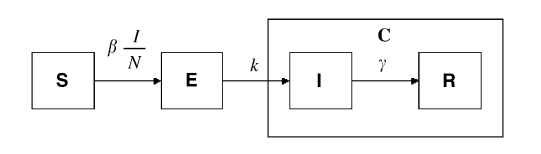
\includegraphics[scale=0.4]{seir_model_fig}
\centering\caption{SEIR model}
\label{fig:SEIR_model}
\end{figure}

In the SEIR model, susceptible (S) individuals in contact with the virus enter the exposed (E) state
at a rate of $\beta I / N$.
The exposed (E) individuals undergo an average incubation period of $1/k$ days before progressing to
the infectious (I) state. The exposed state is assumed to be asymptomatic as well as uninfectious.
Infectious (I) individuals move to the R state, either recovered or dead, at a rate of $\gamma$.
 The parameters are $\beta$, the transmission rate per person per day;
$N$, the total effective population size; and $I/N$, the probability that contact is made with
an infectious individual.

In \citep{legrand2007understanding}, the Ebola outbreaks in Congo in 1995 and Uganda in 2000 are
also studied. However, they expand on the model from \citep{chowell2004basic} by modeling the
spreading of Ebola in heterogeneous settings. In order to gain more insight into the epidemic
dynamics, the infectious phase is subdivided into three stages: infection in a community setting
(I), infection in a hospital setting (H), and infection after death assuming a traditional funeral
(F). The resulting model is known as the SEIHFR model.

A CDC (Centers for Disease Control and Prevention) report \citep{meltzer2014estimating} published
September 26, 2014 makes use of the SEIHFR model to provide an estimate of the future number of cases
of the current Ebola epidemic. While the SEIHFR model provides finer grained modeling of the behavior of
Ebola, it is also complex and the link to a network-based model becomes tenuous. In addition, the
current 2014 Ebola epidemic is still in progress and we do not have the entire picture of the
epidemic cycle. Given the limited number of data points, trying to fit a model with a large number of
parameters may lead to overfitting.  Because of these reasons, we do not plan to use the SEIHFR
model in our work.

\subsection{{Network-based epidemiological model}}

In the compartmental models described in the previous section, the underlying assumption is random
mixing among the population. Therefore, an infected individual can infect any other individual in the
population. Even though \citep{legrand2007understanding} modified the SEIR model to reflect the
heterogeneity of infection states, the underlying assumption is still random mixing. However,
contagious diseases like Ebola spread via networks formed by physical contacts among individuals.
While an individual may have the same number of contacts per unit time in either a random mixing
model or a network contact model, within a static network model the set of contacts is fixed, versus
a random-mixing model wherein it is continually changing. A static network model thus captures the
permanence of many human relationships.

In our search for existing literature on a network-based model for the spread of Ebola, we haven't come
across any previous work that precisely does this, possibly due to the lack of detailed data in the
locations historically affected by the disease.  In \citep{newman2002spread}, the authors provide
the relationship between the compartmental SIR model and a random network model. The author introduces
the concept of transmissibility in a network model. Transmissibility of a disease in a network model
is defined as the average probability that an infectious individual will transmit the disease to a
susceptible individual with whom they have contact. The authors also provide equations that connect
the transmissibility and degree distribution of a random network with the basic reproductive number
of an SIR model.

In \citep{meyers2005network}, the authors model the spread of the 2002-2003 outbreak of SARS in Hong
Kong and Canada using a network model. A contact network model attempts to characterize every
interpersonal contact that can potentially lead to disease transmission in the community. Each
person in the community is represented as a node in the network and each contact between two people
is represented as an edge connecting them. In \citep{meyers2005network}, the authors presented three
different contact network models for SARS -  \textit{(a) Urban Network:} A plausible urban-setting
contact network generated using simulation based on data from City of Vancouver, Canada. Households
were randomly chosen and  their members given ages, schools, occupations, hospital beds as patients,
and  caregivers according to statistics from public data.  This model offers a high degree of
realism, but is complex. \textit{(b) Random Network:} A random network with Poisson degree
distribution in which individuals connect to others independently and uniformly at random.
\textit{(c) Scale-free Network:}  A truncated power law degree distributed network can model
individuals, called ``superspreaders'' with unusually large numbers of contacts or ``supershedders"
who are unusually effective at excreting the virus into the environment they share with others.

%Transmissibility $T$ of a disease in a network model is defined as the average probability that an
%infectious individual will transmit the disease to a susceptible individual with whom they have
%contact. The epidemic threshold $T_c$ is the minimum transmissibility required for an outbreak to
%become a large-scale epidemic.  In \citep{meyers2005network}, authors extended the results from
%\citep{newman2002spread} to provide the relations between the basic reproductive number $R_0$ of an
%SIR network and the transmissibility $T$ and epidemic threshold $T_c$ of a random networks. as
%follows:
%
%\begin{equation} R_0 = T  \dfrac{\left\langle k^2 \right\rangle}{\left\langle k \right\rangle-1},
%\quad\quad T_c =\dfrac{\left\langle k \right\rangle}{\left\langle k^2 \right\rangle - \left\langle
%k \right\rangle} \end{equation}
%
%where, $\left\langle k \right\rangle$ and $\left\langle k^2 \right\rangle$ are the mean degree and
%mean square degree of the network.
%
Neither of \citep{meyers2005network, newman2002spread} captured the temporal progression of the
epidemic using a network model. Instead, the authors provide the final number of infected nodes in a
network for a given value of $T$. Compared to the compartmental model, there are two major drawbacks
in a network-based model:

\begin{enumerate}[(a)] \item The compartmental model is a well-established model and can generally capture
      the temporal progression of disease spread in a localized population fairly well. In contrast,
      with a contact  network, it is hard to model the spread of disease over time. In general,
      percolation theory is used in conjunction with a contact network to predict the final number
      of individuals that can get affected in a given network. However, it is generally hard to
      reliably predict the stage of the disease at a given time with a network model.

\item In general, it is almost impossible to model the actual contacts among individuals. Therefore,
in most network model, many assumptions are made to model the contact network. \end{enumerate}

\subsection{{Combination of a compartmental and a network-based epidemiological model}}

As discussed in previous sections, a compartmental model is convenient in analyzing the temporal
progression of a contagious disease in a localized population. However, due to the underlying
assumption of random mixing among the population, such a model is not suitable for analyzing a large-scale
outbreak of a contagious disease at a world-wide scale. An attractive alternative solution in
analyzing the progression of disease in a world-wide scale is by combining a compartmental and
network model. In such a formulation, the compartmental model is used on a local scale to track the
progression of disease in individual countries (or cities or continents). To capture the dynamics of
inter-country (city or continent) spread of disease, some form of network data can be used. Such
network data are usually converted to inter-country (or city or continent) transfer of population per
unit time.

In \citep{balcan2010modeling} the authors model the inter-country and inter-city spread of
population using airport network data and commuting network data. The authors then use such a model in
conjunction with a stochastic compartmental model to analyze the 2001-2002 seasonal influenza
outbreak. A similar work \citep{gomes2014assessing} attempts to predict the spread of Ebola to
different parts of the world based on a model that incorporates both the compartmental approach and
the use of world-wide air traffic flows. In this model, the world is divided into geographcal
regions defining a subpopulation network, modeling connections among subpopulations representing
traffic flows due to transportation infrastructure.

%%%%%%%%%%%%%%%%%%%% INTRA COUNTRY COMPARTMENTAL %%%%%%%%%%%%%%%

%   Model/Algorithm/Method (30%) + Results and findings (35%)

\section{{Modeling and Analysis of Intra-country Spread of an Epidemic}}
\label{sec:IntraCountry}

\subsection{System Model and Algorithms}
In the first phase of the project, to calculate the basic reproductive number of the current Ebola
epidemic spread in different countries, we performed model fitting on the data we gathered from
\citep{cmriversdata}. We considered the SEIR model described in \citep{chowell2004basic}. The
following set of differential equations are used to represent this model \citep{chowell2004basic}:

\begin{equation}
\dfrac{dS}{dt}	=	\dfrac{-\beta SI}{N},
\quad
\dfrac{dE}{dt}	=	\dfrac{\beta SI}{N}-kE,
\quad
\dfrac{dI}{dt}	=	kE-\gamma I,
\quad
\dfrac{dR}{dt}	=	\gamma I,
\quad
\dfrac{dC}{dt}	=	kE.
\label{Eq:SEIR}
\end{equation}

Here, $S$, $E$, $I$, and $R$ denote the number of susceptible, exposed, infectious and removed
individuals at time $t$. $C$ is not an epidemiological state, however it is useful to keep track of
the cumulative number of infected cases from the time of the onset of the outbreak. In order to
model the effect of intervention on the spread of the disease, in the above model, the transmission
rate $\beta$ is modeled as a function of time. At the initial phase of the outbreak, before
intervention, $\beta$ is parameterized by $\beta_0$. After intervention, the value of $\beta$
transitions from $\beta_0$ to $\beta_1$, $\beta_0>\beta_1$ as follows:

\begin{equation}
\beta(t)=\begin{cases}
\beta_{0} & t<\tau\\
\beta_{1}+(\beta_{0}-\beta_{1})\exp\left(-q\left(t-\tau\right)\right) & t\ge\tau
\end{cases}
\label{Eq:Beta}
\end{equation}

\noindent where $\tau$ is the time when interventions begin and $q$ controls how quickly the rate of
transmission changes from $\beta_0$ to $\beta_1$. The SEIR model under consideration is a non-linear
model with six parameters.

The current Ebola epidemic is still spreading and depending on the preventative measures  taken, the
underlying dynamics of the spread can change drastically any time. The Ebola data for the three
most-affected countries in West Africa - Guinea, Sierra Leone and Liberia - were represented as $(t_i,y_i)$,
$i=1,2,\ldots,n$ where $t_i$ represents the $i$th reporting time and $y_i$ the cumulative number of
infectious cases from the beginning of the outbreak of to time $t_i$.  The model parameters
$\Theta=(\beta_0,\beta_1,k,q,\gamma, \tau)$ for these three countries were estimated using a
non-linear least-squares procedure by fitting these data to the cumulative number of cases
$C(t,\Theta)$ in Equations \eqref{Eq:SEIR}, \eqref{Eq:Beta}. In addition, we performed model fitting
for the West Africa region by adding up the data from these three countries.

Given the limited number of data available, instead of fitting all six parameters to the model, we
decided to fix some of the parameters based on studies on previous Ebola epidemics. In
\citep{chowell2004basic}, the incubation time of the Ebola virus $1/k$ is found to vary between 1
and 21 days, with a mean time of 6.3 days for previous Ebola outbreaks. For ease of data fitting, we
set this parameter value to the mean value of 6.3 days. We note that the dynamics of the current
epidemic may differ from previous ones, and therefore fixing a value based on the prior estimate may
lead to some inaccuracy.  The choice of selecting initial outbreak time $t_0$ and intervention time
$\tau$ is a difficult problem. To this end, we looked into different sources like WHO (World Health
Organization) and CDC websites to learn more about the timeline of the spread. In Guinea, a
2-year-old boy died on December 2, 2013, later diagnosed as an Ebola patient. We consider this
incident as the index case for Guinea and set $t_0$ to December 2. On March 2, the Government of
Guinea informed WHO regarding the possibility of an Ebola epidemic and declared a national heath
emergency. We considered this date as the intervention date and set $\tau$ to 110. In Sierra Leone,
one person died on April 2014. In June 12, 2014 the country declared an emergency and closed its
borders with neighboring Guinea and Liberia. We consider the first date as $t_0$ and second date as
the intervention time, therefore set $\tau$ to 50. In Liberia, on March 31, 2014, there was official
confirmation of two people infected with Ebola. We set this date to $t_0$ and set $I_0$ and $C_0$ in
our model as 2. The government of Liberia shut down all schools on July 30, 2014. We consider this
date as the date of intervention in Liberia and set $\tau$ to 120.

%In order to fit the non-linear SEIR model to the data, we used non-linear least squares estimation.
%We use the reported data $(t_i, c_i)$ for $i=1,2,\ldots,n$ where $t_i$ denotes the $i-th$ reporting
%time and $c_i$ the cumulative number of infectious cases from the beginning of the outbreak at time
%$t_0$ to time $t_i$.

The optimization problem involving the model fitting of the SEIR model is a non-linear least squares
regression problem and contains a large number of local minima. Therefore, the choice of initial
parameter estimate is an important consideration to get a globally optimal solution. In order to
find a good initial choice of the parameters as input to the non-linear least squares solver, we
first perform a Latin hypercube sampling on the  4-dimensional parameter space.  We grid up the
hypercube with a number of grid points in each dimension.  We then choose the sample that minimizes
the least squares error as the initial input. In order to calculate the 95\% confidence interval of
the estimated parameter, we performed bootstrapping based on residual error.

\begin{figure}[ht]
\centering
\subfigure[Guinea]{
  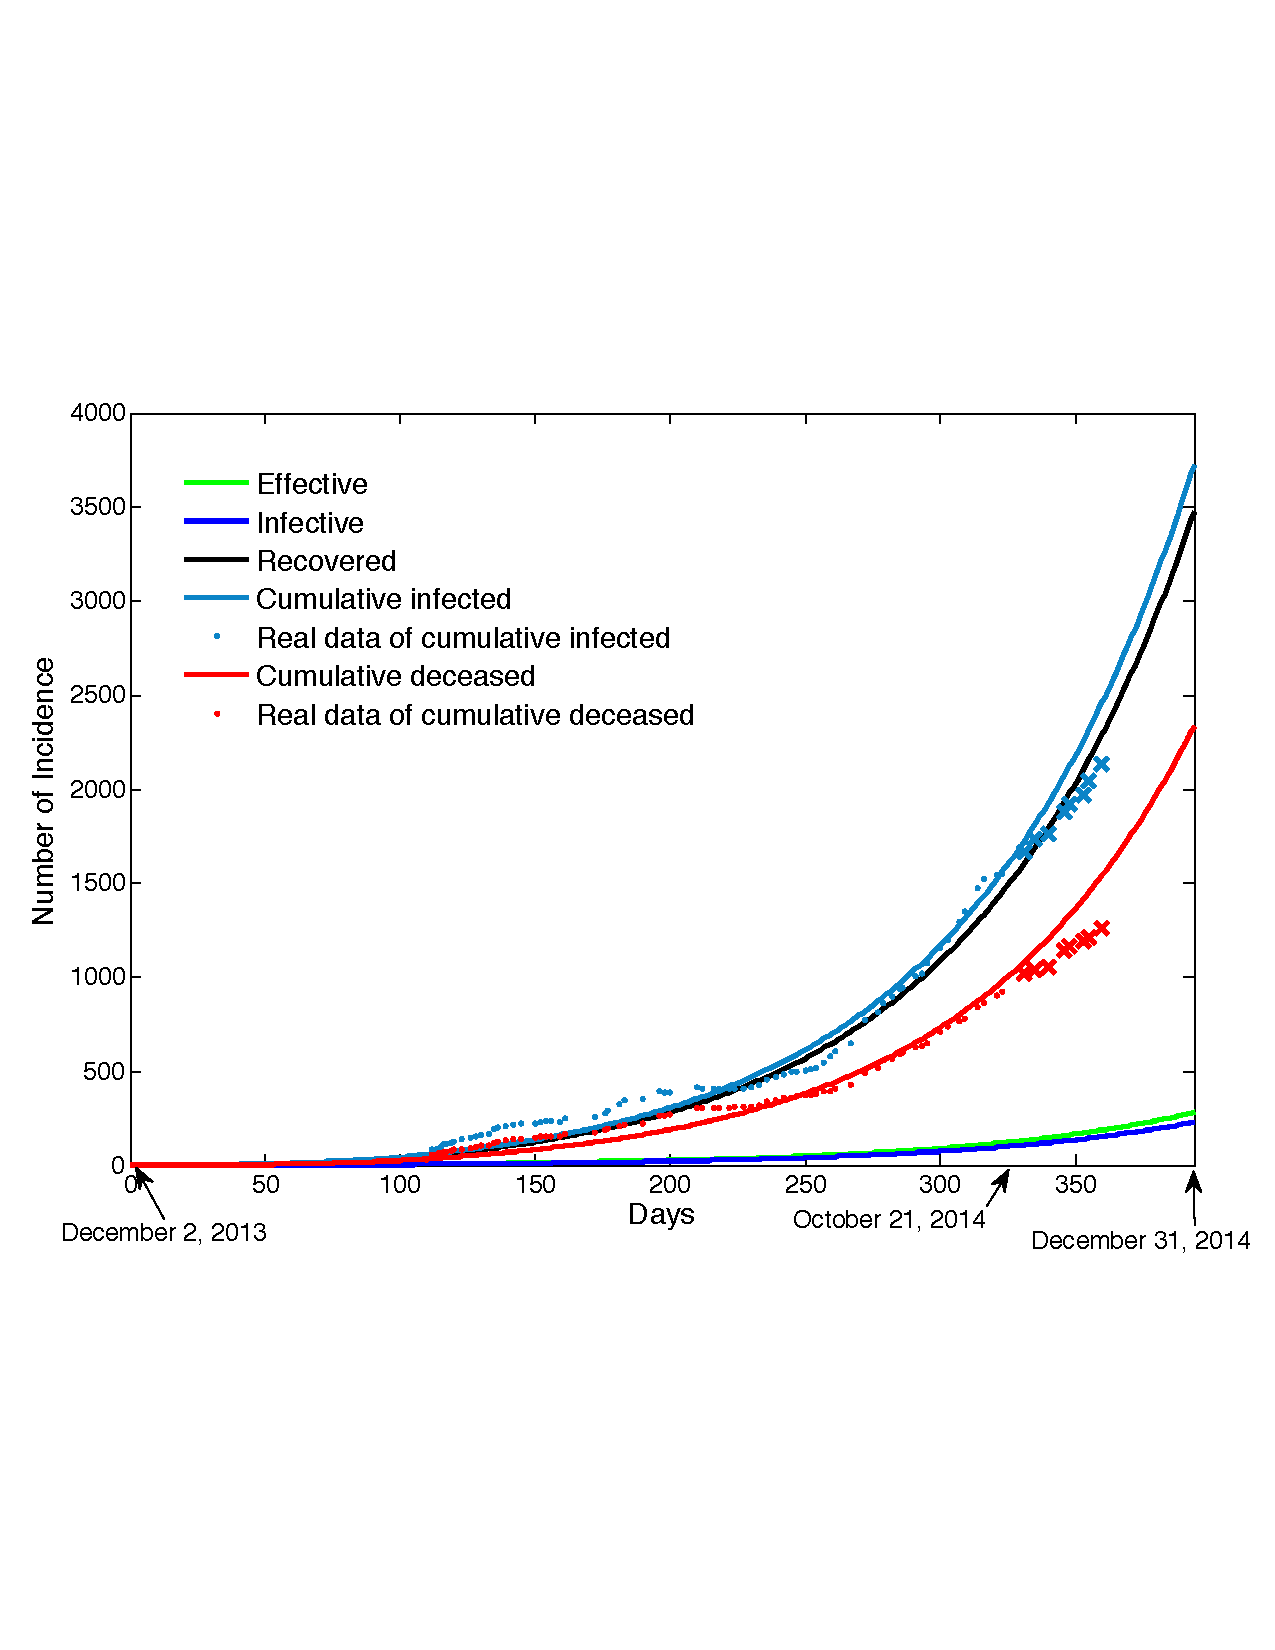
\includegraphics[width=0.45\textwidth]{Guinea1.pdf}
  \label{fig:subfigure1}}
\quad
\subfigure[Sierra Leone]{
  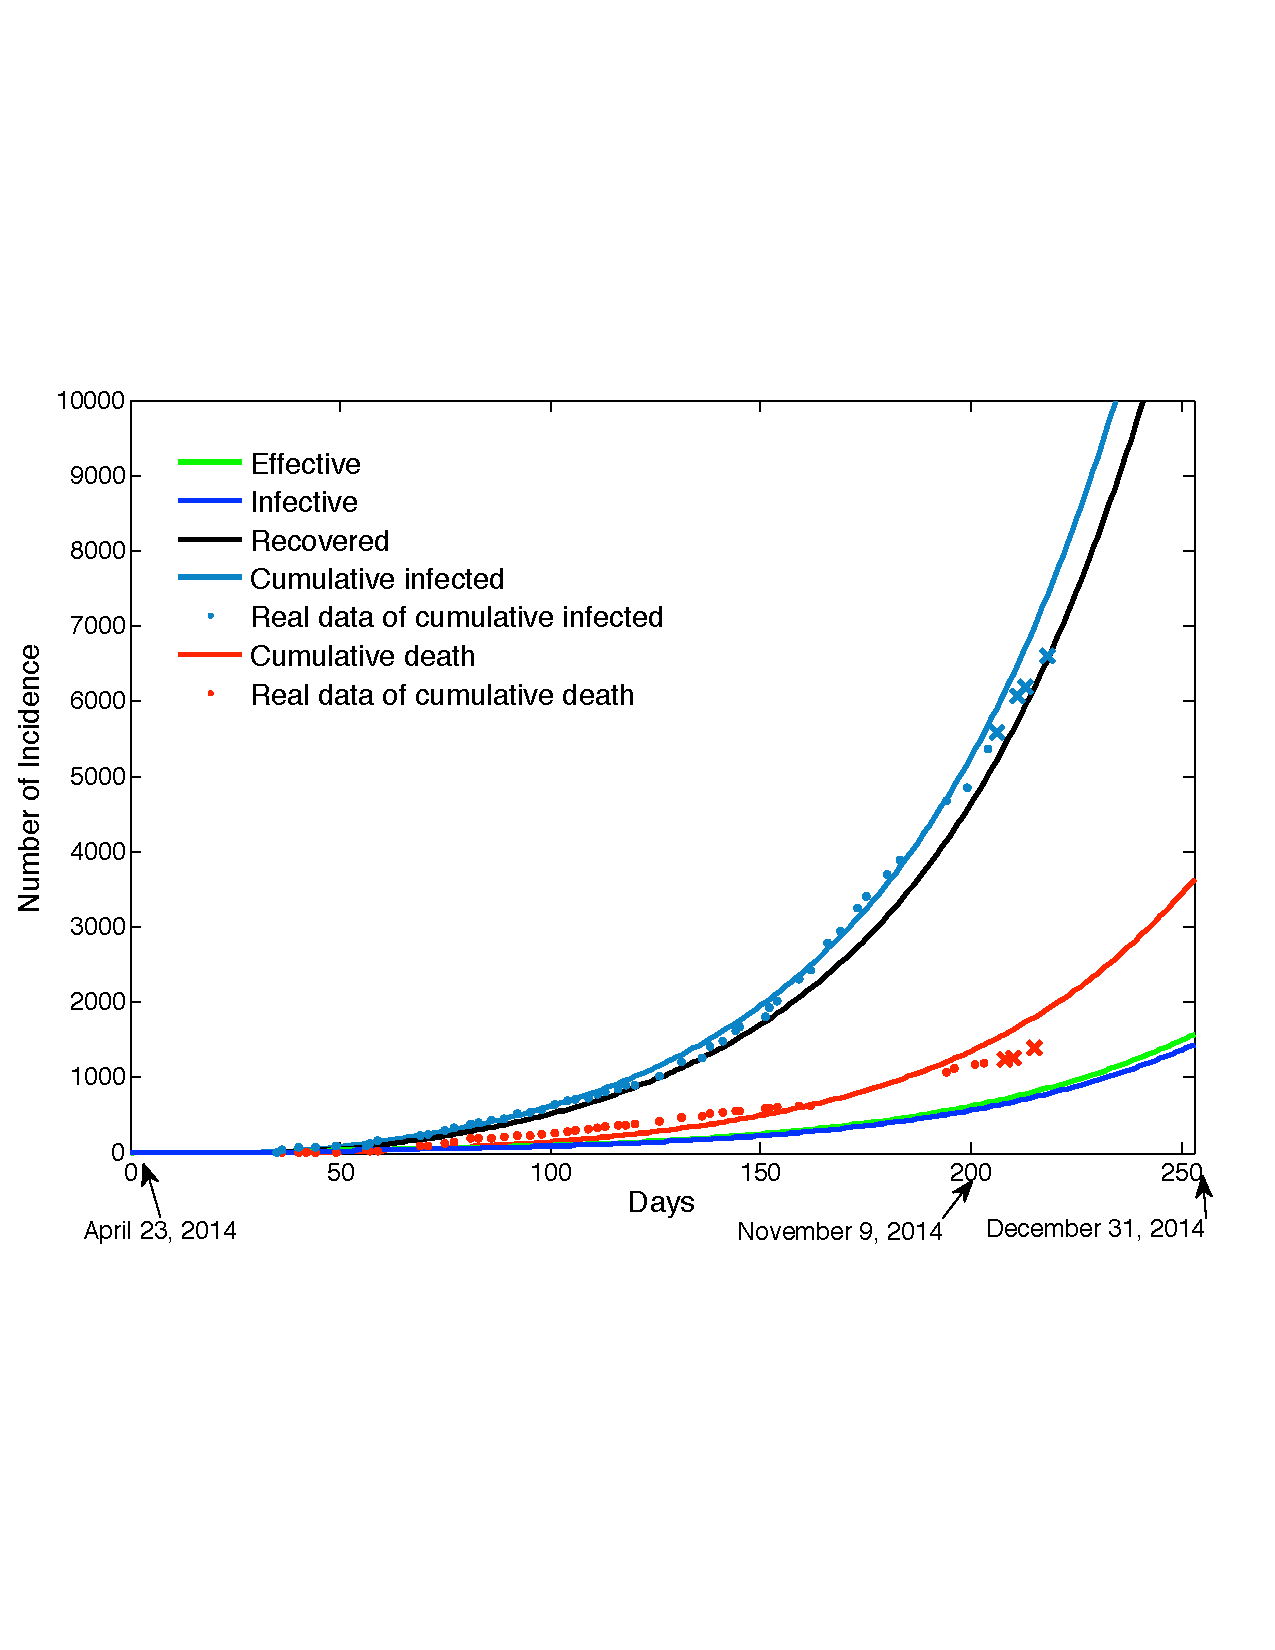
\includegraphics[width=0.45\textwidth]{SierraLeon1.pdf}
  \label{fig:subfigure2}}
\subfigure[Liberia]{
  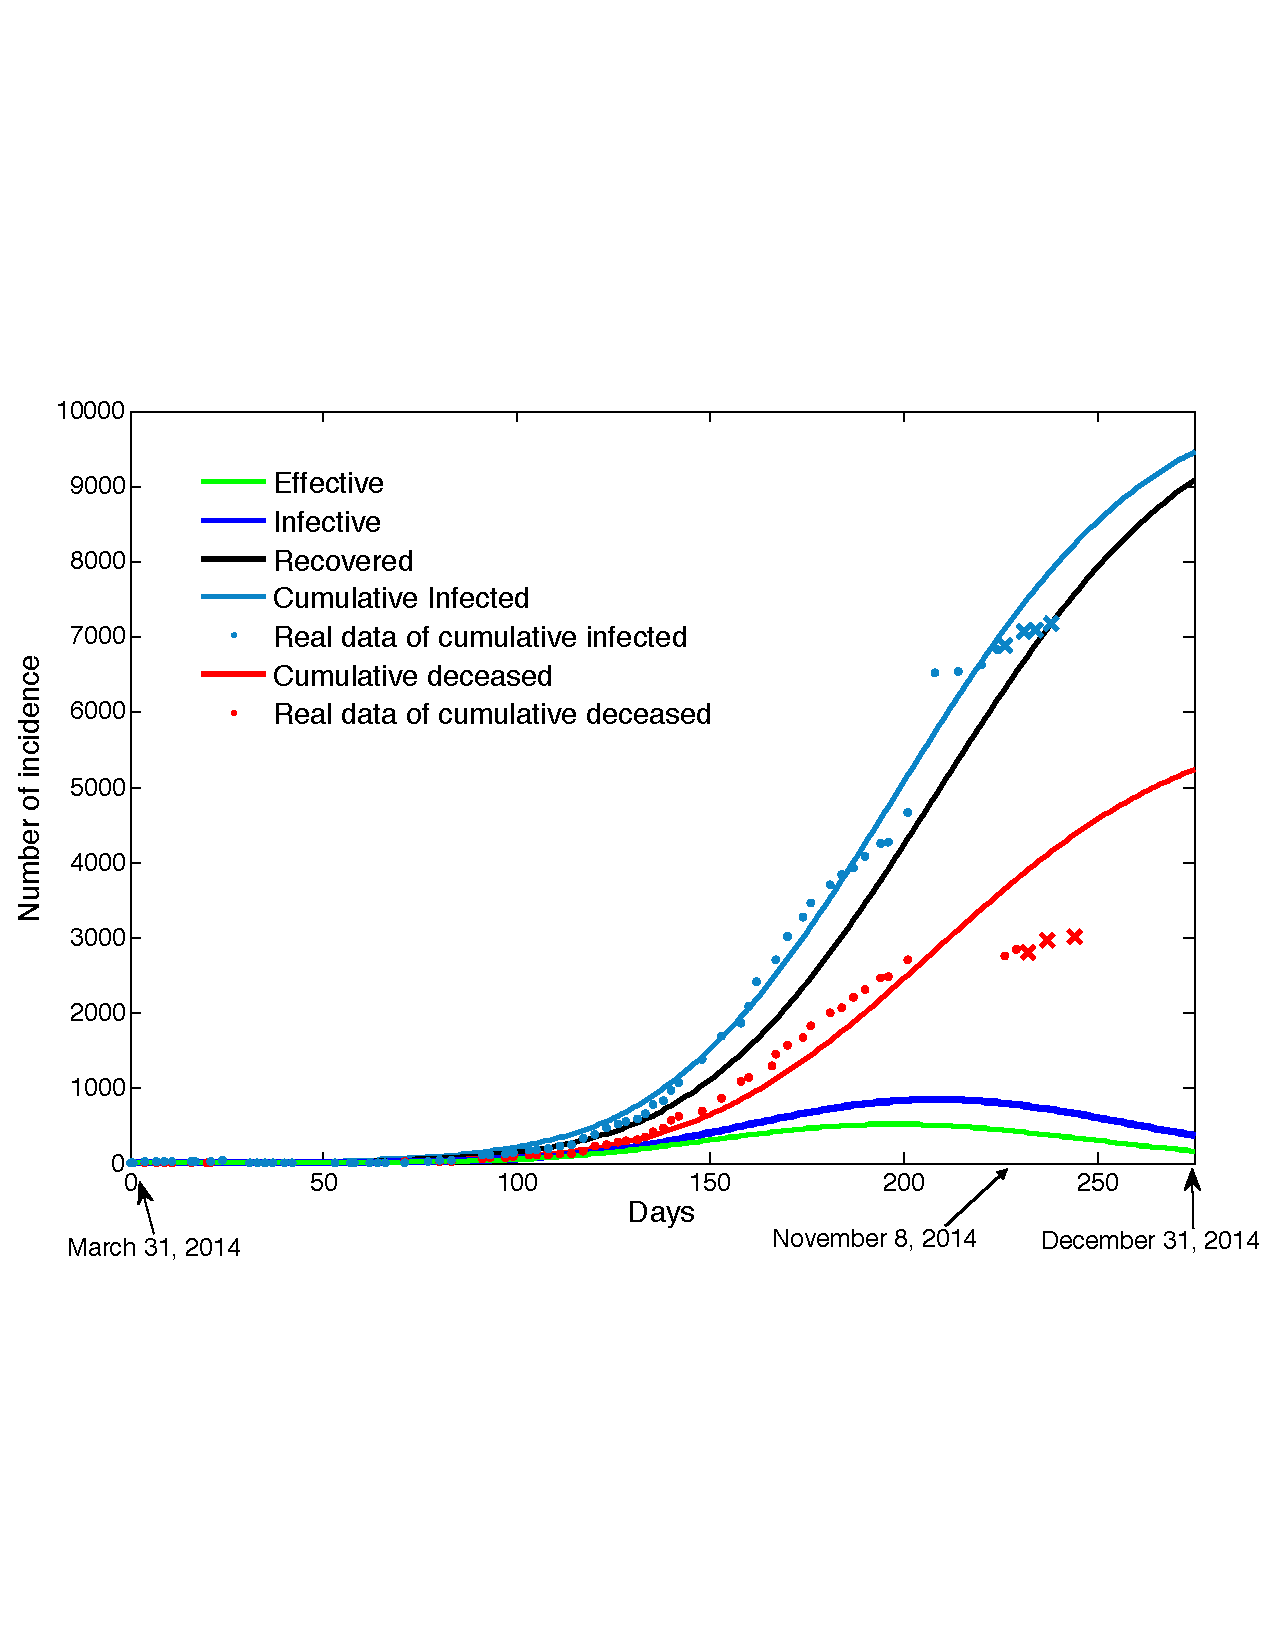
\includegraphics[width=0.45\textwidth]{Liberia1.pdf}
  \label{fig:subfigure3}}
\quad
\subfigure[West Africa]{
  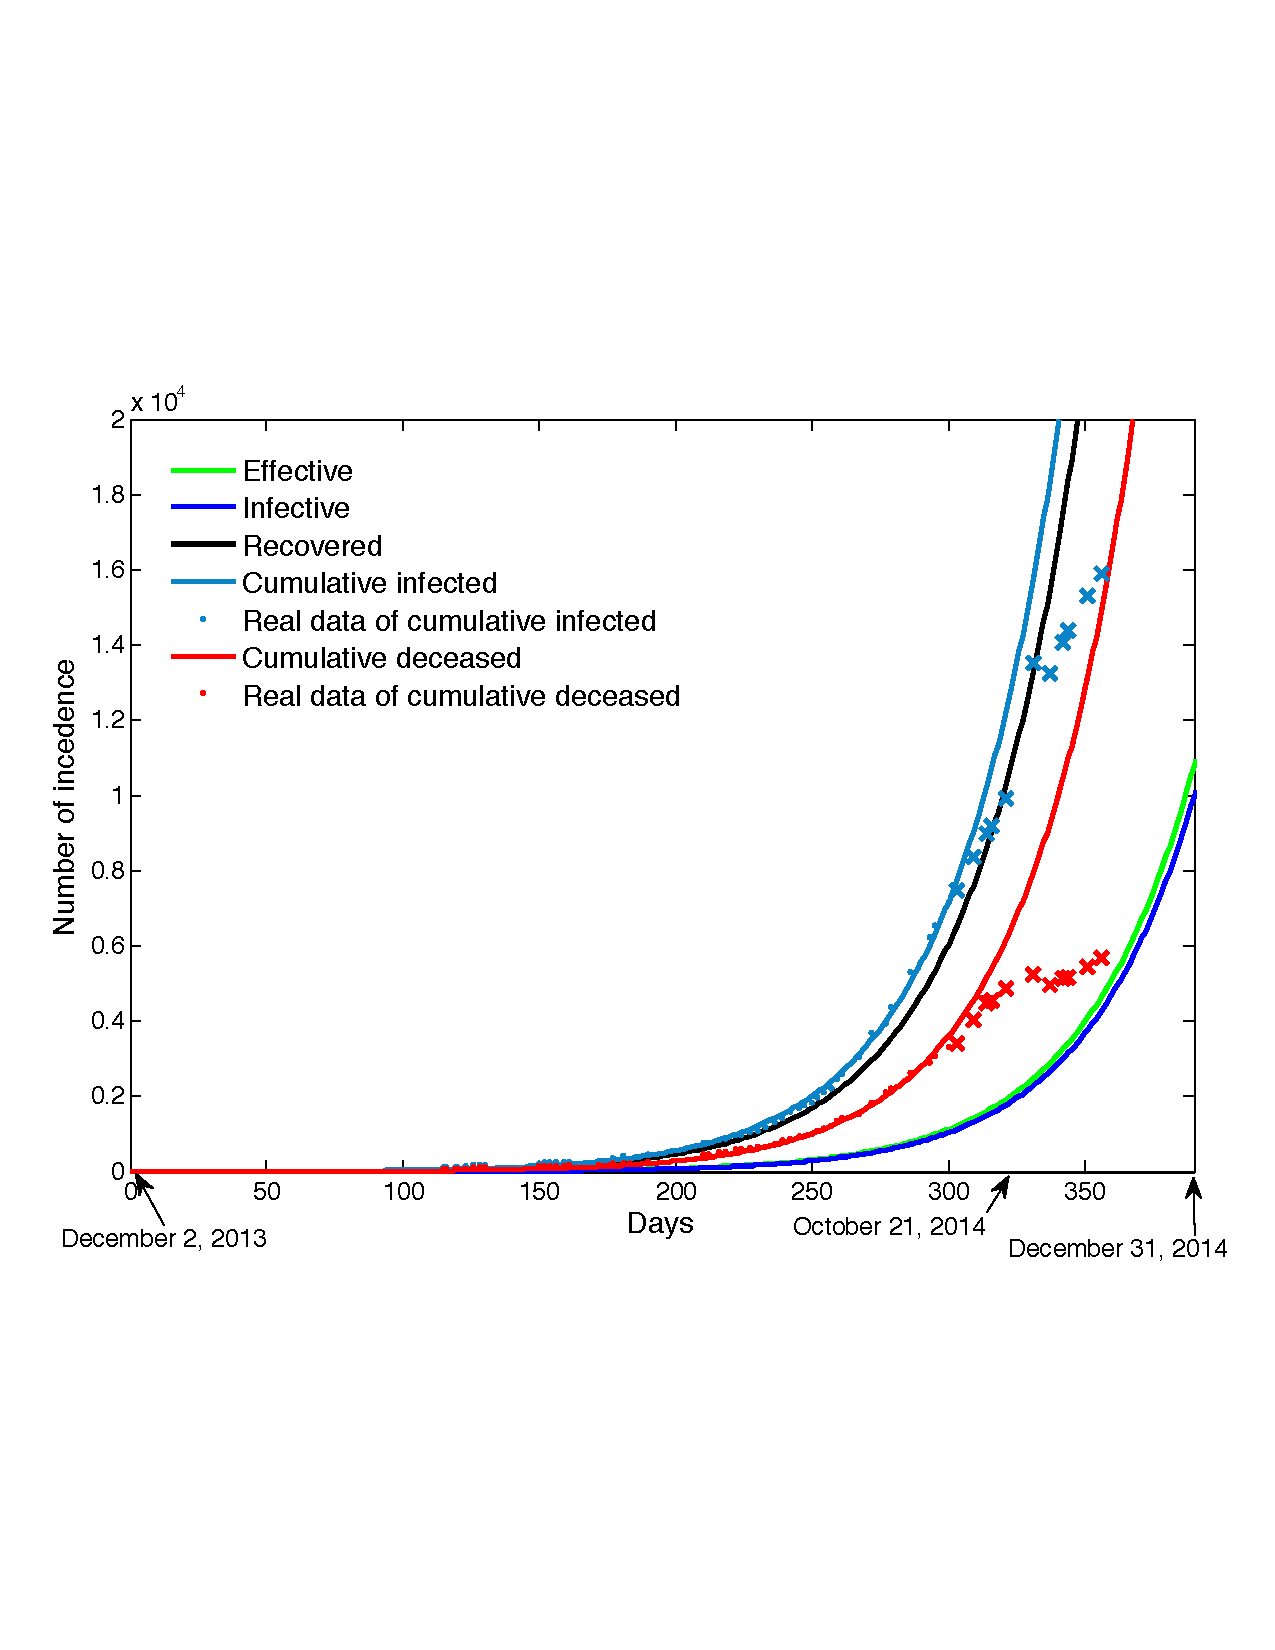
\includegraphics[width=0.45\textwidth]{WestAfrica1.pdf}
  \label{fig:subfigure4}}

\caption{SEIR model fit results for 2014 Ebola epidemic data}
\label{Fig:figurePrediction}
\end{figure}


\subsection{Results and Findings} The estimated parameters for the SEIR model of Guinea, Sierra
Leone, Liberia, and the overall West Africa region is presented in Tables \ref{Table:parameter} and
\ref{Table:parameter2} in the Appendix. The basic reproductive number of the epidemic before and after
intervention, $R_0 \approx \frac{\beta_0}{\gamma}$  and $R_1 \approx \frac{\beta_1}{\gamma}$ for the
three countries are also presented in the tables. In Figure \ref{Fig:figurePrediction}, we presented
the number of incidents at different compartments of the SEIR model, as well as the cumulative
number of infectious cases over time. In our project milestone report, our model fit was based on
the last data we collected on Oct. 21, 2014. At the time of writing this final report, we have
additional data points available. Based on data collected till November 9, 2014, we have updated our
parameter estimation for Sierra Leone and Liberia. We, however, kept the same model for Guinea as in
our milestone report, since we have the most amount of data available for Guinea already due to an
earlier outbreak date in Guinea (Dec. 2, 2013). We extrapolated the graph up to Dec. 31, 2014.  We
note that forecasting future cases may not be accurate as the underlying factors of the epidemic are
changing rapidly with the increase in safety measures. The unused data for Guinea (Oct. 21 - Dec.
5), Sierra Leone (Nov. 10 - Dec. 5) and Liberia (Nov. 10 - Dec. 5) are used for calculating test
error. These values are also plotted in Figure \ref{Fig:figurePrediction} (points represented with
`.' sign are used for training, points represented with `x' sign are used for testing). We observe
that the predictions of the model to the cases up to Dec. 5 are mostly on par with the observed data
for Guinea, Sierra Leone and Liberia. For the Guinea epidemic, we have data for the longest range of
days and the estimated model, therefore, captures most of the dynamics of the spread in contrast to
the other cases.

For the West Africa region plot, our prediction number is much higher than the actual data. This is
understandable, as the underlying assumption behind the SEIR model is random mixing.  Within a
country without any movement restriction, this model is somewhat appropriate. However, for the
aggregated model among multiple countries, this assumption is no longer valid due to stricter
movement regulations between country borders. Therefore, a model with a random mixing assumption
will overestimate the number of infectious cases.


\begin{table}[h]
\caption{Estimated number of total infected people (by December 31, 2014) and root mean square error (RMSE) of prediction}
\centering
\begin{tabular}{|c|c|c|c|}
\hline
Country & Estimated Number of Infected individuals & Cross-validation Error & Test Error
\tabularnewline
\hline
\hline
Guinea & 3724 & 100.96 & 218.9\tabularnewline
\hline
Sierra Leone & 14040 & 170.14 & 546.2\tabularnewline
\hline
Liberia & 9500 & 350.3 & 504.24\tabularnewline
\hline
\end{tabular}
\label{Tb:prediction}

\end{table}

In Table \ref{Tb:prediction}, we presented our estimate of the total number of people who could get
infected by December 31, 2014 as well as root mean square cross-validation error of our model fit
and test error on the unused data.


\section{Analysis of Network based Epidemiological Model} \label{sec:NetworkModel}


\subsection{{Problem Definition and Algorithms}}

In Phase II of our project, we attempt  to map the compartmental model to network based model  using
percolation theory to model the spread of Ebola in West Africa. The mapping between a compartmental
model and a network based model is defined in \citep{meyers2005network}.Transmissibility $T$ of a
disease is defined as the average probability that an infectious individual will transmit the
disease to an individual with whom they have contact. Critical transmissibility or epidemic
threshold $T_c$ is the value of transmissibility above which a population is vulnerable to large
scale  epidemics when the basic reproductive number $R_0$ is 1. For our analysis, we reused the
following expression from \citep{meyers2005network}:

\begin{equation}
R_0 = T  \dfrac{\left\langle k^2 \right\rangle}{\left\langle k \right\rangle-1},
\qquad\qquad
T_c =\dfrac{\left\langle k \right\rangle}{\left\langle k^2 \right\rangle - \left\langle k \right\rangle}
\label{eq:transmissibility}
\end{equation}

For simulating a contact network for Ebola in various infected countries we used a data set from a
social networking site available on \citep{topcoderdata}. The undirected network has 4,846,609 nodes
and 42,851,237 edges and average degree of $8.841$. The network exhibit a power law degree
distribution after a degree of approximately 50. We also generated three other datasets  for a
preferential attachment network, random network and a small-world network with approximately same
number of nodes and average degree as the real network for comparison purposes.

Transmissibility values for each of three infected countries Liberia, Guinea and Sierra Leone in
West Africa are calculated using Equations \eqref{eq:transmissibility}  and the reproductive number
from Table \ref{Table:parameter}, \ref{Table:parameter2}. These values are presented in Table
\ref{tab:T}.  We calculated the epidemic threshold  $T_c=0.1275$  using k=8.841 and used these
values for  running the simulations on the  network datasets.


\begin{table}[h]
\caption{Transmissibility values for  Liberia, Guinea and Sierra Leone}
\begin{center}
    \begin{tabular}{ | l | l | l | p{5cm} |}
    \hline
    Country & $R_0$ & Transmissibility(T) \\ \hline
    \hline
    Liberia & 0.001 & 0.001  \\ \hline
    Guinea & 1.145 & 0.1148 \\ \hline
    Sierra Leone & 1.24 & 0.1243  \\ \hline
    \end{tabular}
\end{center}
\label{tab:T}
\end{table}
\label{Tb:Transmissibility}

Since our datasets were  large and simulation using a percolation model is a compute intensive
process, it was not possible to run the simulations in a reasonable time on a local machine so
we ran our simulations on a c3.8xlarge Amazon EC2 instance. Our simulations needed to run for
multiple values  of transmissibility so we developed a test harness written in python
to parallelize computation process-wise and leverage multiple cores on the machine.
Our simulation using  all
four datasets and 20 different values of T  completed in  about 7 hrs for 200 iterations. We also
ran another simulation to see the impact of minimum degree for patient zero for a given
transmissibility value for two different networks.

\subsection{{Results and Conclusion}}

\begin{figure}[ht]
\centering
\subfigure[Transmissibility]{
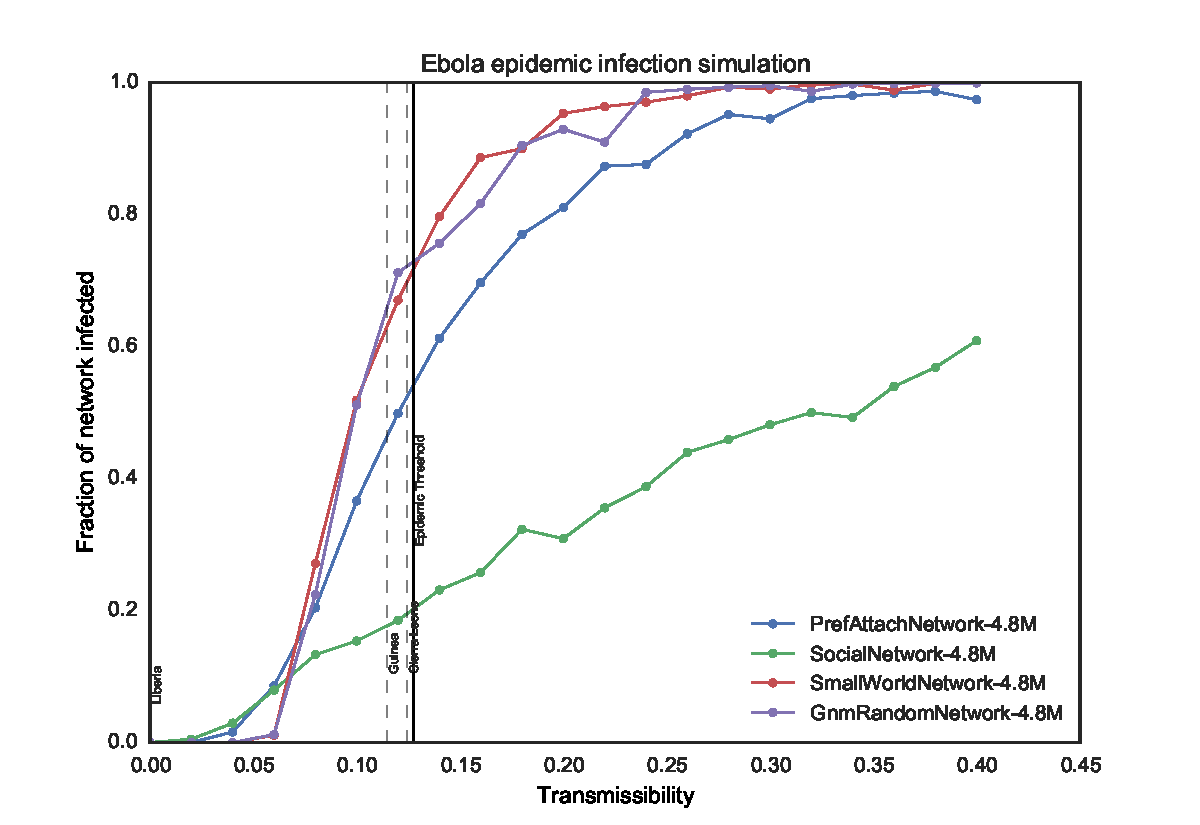
\includegraphics[width=0.47\textwidth]{EbolaNetworkSpread.pdf}
\label{Fig:Network_Transmissibility}}
\quad
\subfigure[Patient Zero Minimum Degree]{
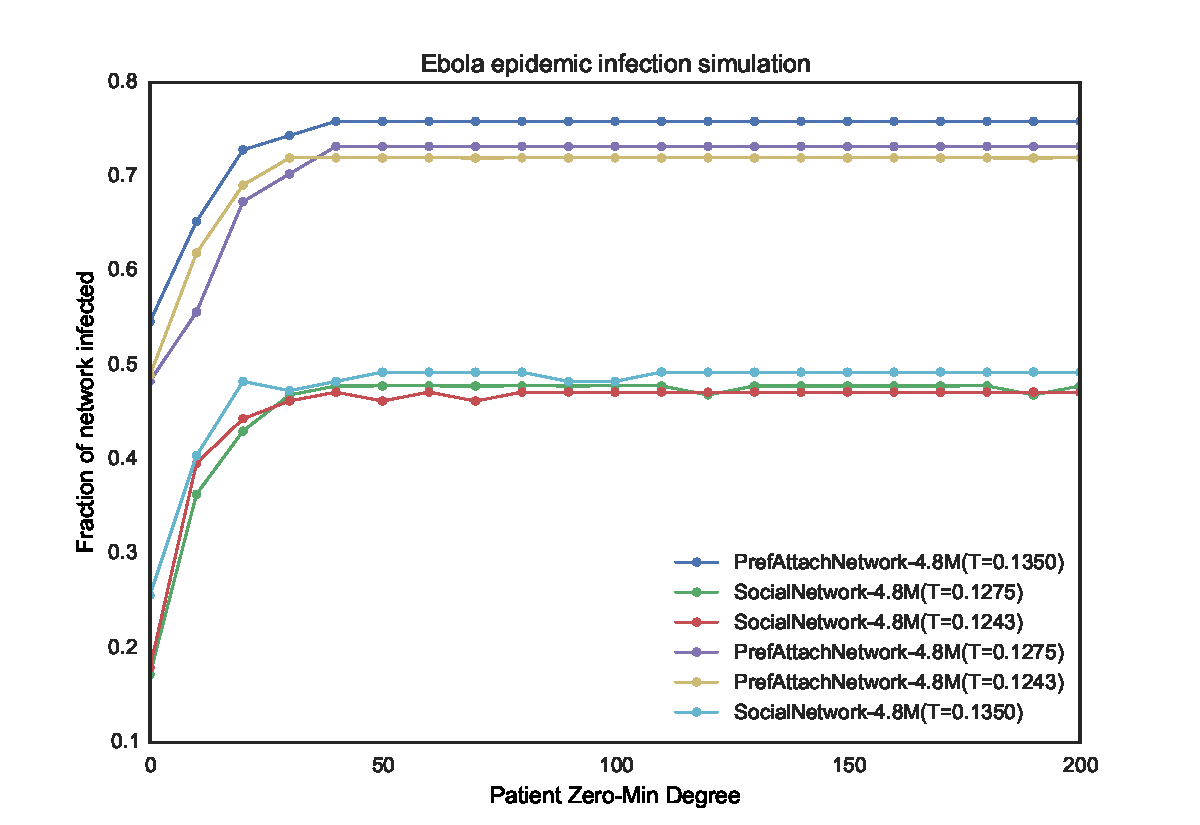
\includegraphics[width=0.47\textwidth]{EbolaMinDeg.pdf}
\label{Fig:Network_MinDegree}}
\caption{Network Simulation for (a) Transmissibility, (b) Patient Zero Minimum Degree}
\end{figure}

In Figure  \ref{Fig:Network_Transmissibility}, we show the fraction of network infected for
different values of transmissibility for  various network types.  The simulation captures the
overall fraction of network infected  but does not capture any temporal progression for Ebola. Above
the epidemic threshold the rate at which the  fraction of the network gets infected increases for
all network types and the rate is higher for other networks in comparison to power law networks
which leads to a conclusion that Ebola outbreak is less likely to become an epidemic in these
networks . This is contrary to the compartmental model assumption that an outbreak will always
become an epidemic when reproductive number is greater than 1. For preferential attachment,
small-world and random networks for value of T in the range of 0.35-0.40 nearly the entire network
gets infected but not the real network.

In Figure \ref{Fig:Network_MinDegree}, we show that  for networks with power law degree
distribution[also know as scale free networks], the fraction of the network getting infected is not
entirely dependent on the minimum degree of the  initial node[patient zero] but also on
transmissibility value. This is owning of the fact that the power law networks have majority  of
nodes with few edges or low degrees and small minority of nodes with high degrees or super
spreaders. Since these high degree nodes are rare, outbreak at low transmissibility values  may fail
to reach these nodes. At higher transmissibility values above epidemic threshold, probability of
reaching the super spreaders is higher leading to higher fraction of network getting impacted.The
fraction become constant after a certain degree distribution, in our simulation around 50 since our
real network follows the power law distribution approximately at degree 50. For predicting the total
number of cases based on the network simulation we assume that a  network similar to our real
network exists in Guinea and Sierra Leone.Using a scaling factor proportional to the population we
predict the total number of people infected at the current transmissibility value using the product
of population, scaling factor and fraction of network infected.
In Table \ref{Tb:prediction_networkm} we present our results. \begin{table}[h]
\caption{Estimated total number infected people}
\centering
\begin{tabular}{|c|c|c|c|}
\hline
Country[Population] & Scaling-Factor & Fraction-of-Network-Infected & Total-Infected-People
\tabularnewline
\hline
\hline
Guinea[11.75M] & 0.6545 & 0.178 & 136,889\tabularnewline
\hline
Sierra Leone[6.2M] & 0.3454 & 0.192 & 41,117\tabularnewline
\hline
\end{tabular}
\label{Tb:prediction_networkm}

\end{table}




We did not have access to the  contact network for the countries  severely impacted by Ebola in 2014
to compare our result with actual values.  It will be  very interesting to infer the hidden network
using the cascade diffusion model based on the data available. Running simulations on  the inferred
network and comparing  with the actual results can provide better insights into the spread of
current epidemic. The transmission probabilities and other heuristics developed can be used for
future analysis.



\section{Predicting worldwide spread}
\label{sec:Worldwide}

\subsection{{Problem Definition} - needs updating}
In order to simulate how the Ebola epidemic might spread across the world, we have assembled a
worldwide network based on international trade. Because the trade numbers are in US dollars,
we have assumed a linear relationship between exports in dollars and travelers going abroad.
This is a strong assumption, and we are considering more sophisticated mappings.
We are using this as a long-range network representing trade-based population movement and
connecting localized subnetworks with these trade-driven edges. We are developing a simulation
framework to run in discrete time steps and predict the spread of Ebola across this worldwide network.

\subsection{{Trade network data preparation}}
\label{SubSec:TradeData}

The trade network dataset we are using is based on data retrieved from the
UN Comtrade database \citep{uncomtradedata} via their web service API.
The data queried for were country-to-country SITC-1 exports from the latest data available
for each country.

Several problems with this raw dataset immediately became apparent which required working around.
Many war-torn countries such as Liberia have not reported detailed export data
to the UN in decades (Liberia last reported in 1984). As a result of this, the export totals
are incorrect for the present day. In addition, this old data reports exports to countries that
no longer exist, including East Germany and Yugoslavia. In order to make the dataset usable for
modern-day predictions, we performed the following transformations on the data (using Perl scripts):

\begin{itemize}
\item Manually remapped non-existent countries to their modern equivalents.
      In a few cases, we had to do a best-effort mapping. For example, Yugoslavia split into many
      states, so we assign exports to historical Yugoslavia to modern-day Slovakia,
      since Slovakia currently has the largest economy of the states that once comprised Yugoslavia.
\item Removed exports from states that no longer exist, preferring export data from
      modern equivalents.
\end{itemize}

We then needed to make the per-country exports sum up to the latest available export data.
The United States \citep{ciatotalexports} World Factbook contains up-to-date export totals
for most countries in the world. Using the above data set, on the (admittedly strong) assumption
that the export distribution
from country-to-country in the UN Comtrade data set has remained the same between the last year a
country has reported detailed export data and the latest totals from the CIA, we linearly renormalized
each outgoing edge in our data set so that the total sum of exports equalled the latest CIA data
for each country.
This required a manual step of mapping country names in the UN dataset to those used in
the CIA dataset.

Once we had a ``renormalized'' dataset including detailed export edges and totals matching
the latest available data, we needed to map these numbers to theoretical international travelers.
We could not find complete, or even nearly complete, publicly available data on the number of
international outgoing travelers per country. While inbound tourism numbers are available from
\citep{worldbankinboundtourism}, for the outbound tourism numbers from \citep{worldbankoutboundtourism},
many countries are missing,
especially the African nations that we care so much about from an Ebola outbreak perspective.
Some data are available from the \citep{unwtooutboundtourism}, however they appear to be behind a paywall.
Data for total air travellers are available from \citep{worldbankairpassengers},
however this total includes domestic flights and so is less useful for our purposes.
While it may have been possible to attempt to get this proprietary data via some other route,
we chose to spend our time getting local data and running simulations instead.

Our approach to map outbound dollars to outbound travelers is to assume a linear relationship
between these numbers, and also to assume that the same linear relationship holds for imports to
inbound tourists to a country.
We currently use the United States as a model and use the ratio of
imports to the United States per year to the number of tourists visiting the United States per year.
Based on data from the \citep{usinboundtourists}, 69.77 million people visited the United States in 2013.
According to our renormalized data set, total imports into the United States were
\$$2.21$ trillion during the same period. Dividing imports by visitors (an admittedly
simplistic approach) gives us a scaling factor of approx. $31,665$. Therefore we have applied this
scaling factor to all edges in our international exports network, giving us some approximation of
outbound travellers from country to country based on export numbers.
While this is a coarse approach, one benefit of this simple method is that it may help capture non-flight-related
travel. Interestingly, the trade network-based approach turned out to be fairly useful and helped us generate
some interesting results.

We show a subset of the trade network in Figure \ref{Fig:worldtrade}, specifically the top 10
trading partners for the three countries currently affected by the epidemic: Guinea, Sierra Leone,
and Liberia.

\subsection{{Supplementing the trade network with local migration}}
\label{SubSec:LocalData}

In order to model local migration for cases where the economic impact is low,
we also approximate population movement across land borders.
The length of the land border between each country is available from
\citep{cialandboundaries}, and the population of each country is available from \citep{ciapopulation}.
We wrote scripts to normalize the country names and come up with an estimate of population movement
across borders for each country due to commuting. Commute data between two given countries is not very
readily available, except for certain regions with a high amount of cross-border commuting.
One such data source is \citep{statnord}, which provides cross-border commute statistics for Nordic countries.
This database shows that approximately .12\% of Denmark workers commute to Norway, while approx. .01\% of
Norwegian commuters commute to Denmark. Due to the open borders between these countries, the number for
Denmark to Norway is probably on the high side overall, and due to the disparity in numbers, the traffic seems
clearly one-way. Based on looking at the generated data, we assumed that the average number of workers worldwide
that commute to another country is 0.02\%.
We assume roughly 50\% of a population of a country is employed;the rest are
children, the retired, homemakers, the unemployed, etc.

Based on the above assumptions, for each country we multiply population times .5 * .0002
= .0001, giving us the number of daily commuters, and then we split that across neighboring
countries proportional to their share of land border lengths. This provides an estimate
of daily cross-border commuters per country, which we use to connect neighboring per-country
networks with edges corresponding to that many commuters.


\begin{figure}[ht]
\centering
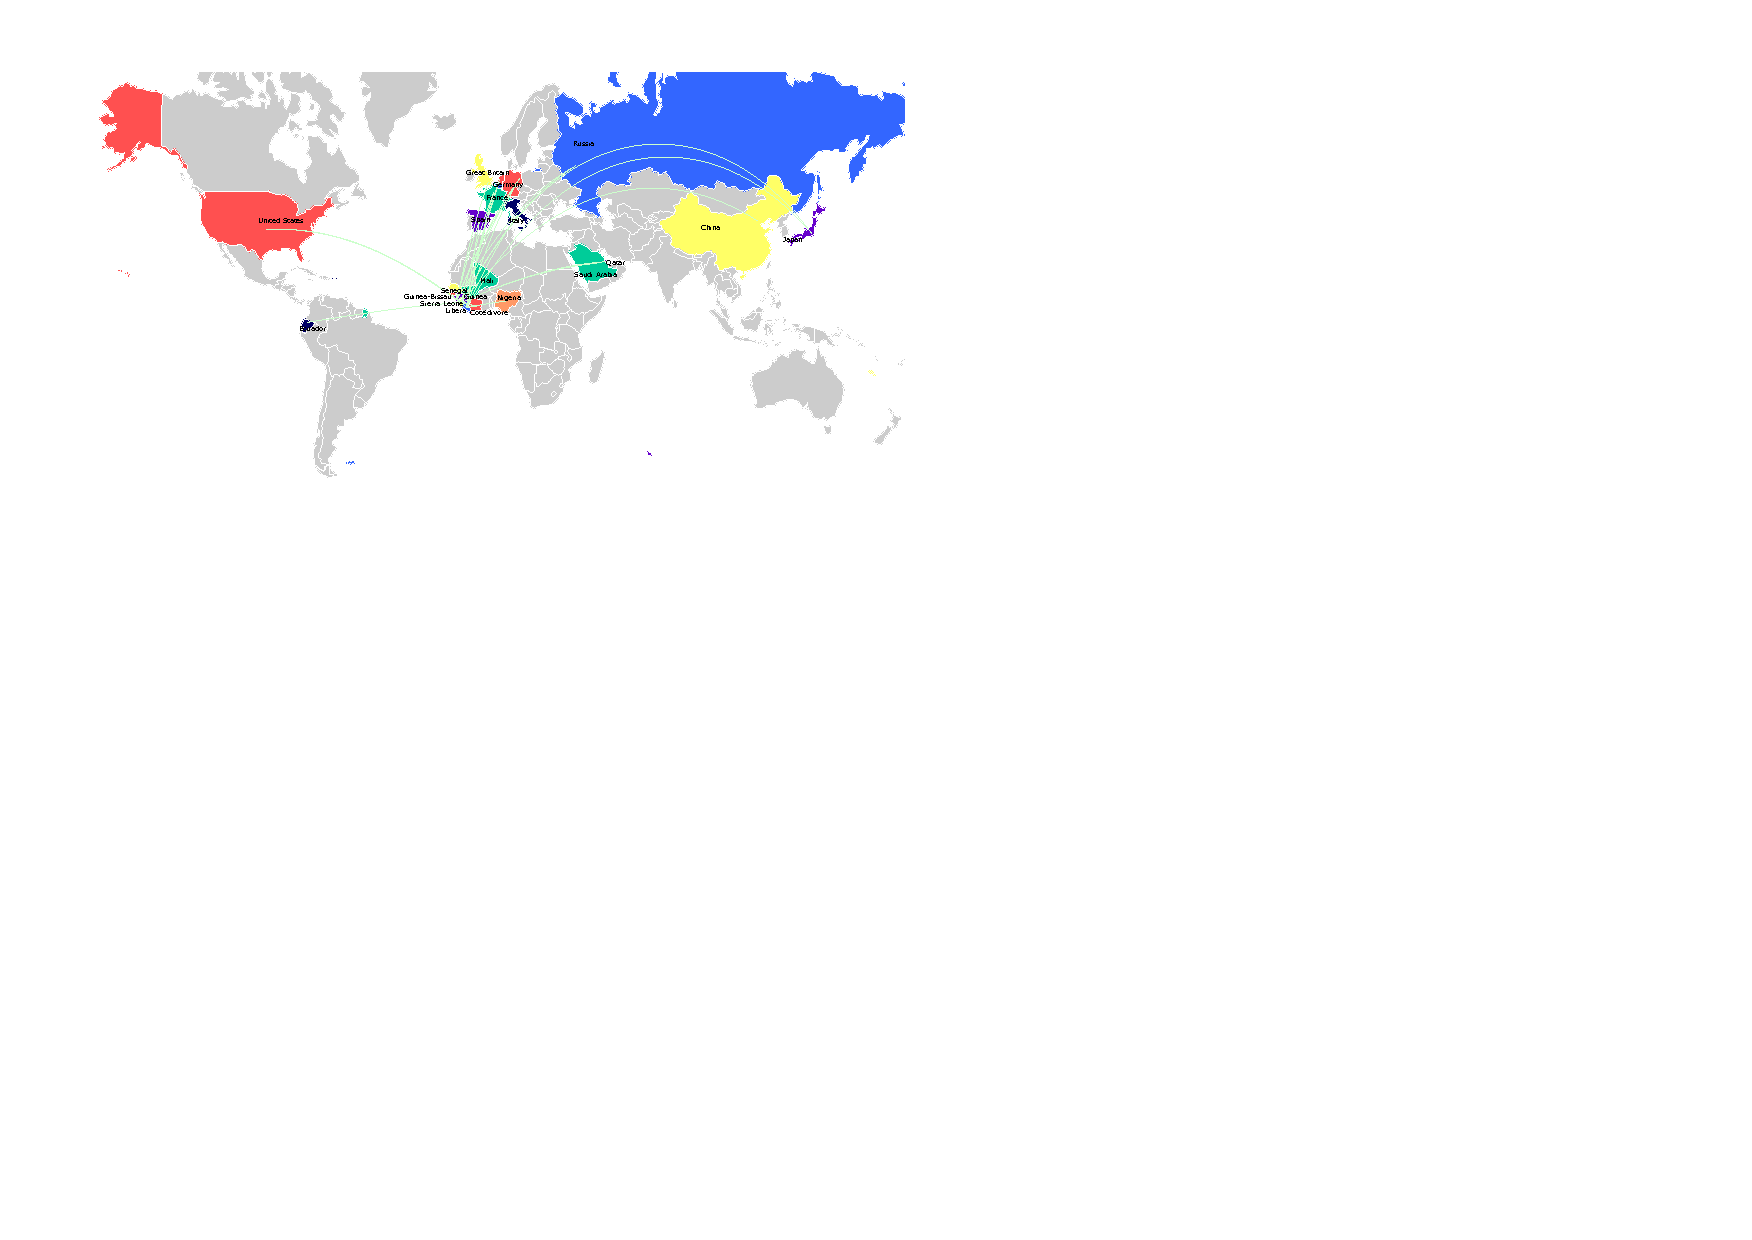
\includegraphics[scale=1.1]{world1.pdf}
\caption{World-wide trade network from Guinea, Sierra Leone and Liberia}
\label{Fig:worldtrade}
\end{figure}


\subsection{{Network Simulation using the SEIR Model}}
\label{SubSec:GraphX}

We also did large-scale experiments on two 25M node "global" networks representing the population
of the Earth, with subnetworks per country. This networks represent a scaled-down version of the
population of the Earth, with a subgraph for each country, number of nodes per subgraph proportional
to the population of that country, and number of edges connecting each subgraph based on the
international migration numbers calculated in Sections \ref{SubSec:TradeData} and \ref{SubSec:LocalData}.

The first global network we built was based on the real-world network from \citep{topcoderdata},
which is a 4.8 million node undirected social network with an average degree of 10. We built each country
as a subgraph based on this network. China, the most populous country with 1.36 billion people
\citep{ciapopulation}, was represented as the full social network, without removing any nodes.
This scale-down factor, of 1.3 billion to 4.8 million, was 279.72.
For each successive country we removed random
nodes from the social network to get it to the right scale relative to China (for example, India
was represented by 4.4 million nodes. The final global graph ended had 25,649,313 nodes.
We then wrote scripts to renumber the nodes in these subgraphs to form a unified global graph.
We added edges beween each subgraph according to the migration numbers calculated previously
(the sum of the trade network and border numbers),
selecting nodes from within each country's respective subgraph randomly.
Finally, we added a self-edge for each node, which allowed us to implement time-stepping and
state-based node transitions without receiving a message from another node within the simulation
environment's Pregel-like algorithm \citep{malewicz2010pregel}.
The resulting number of edges for this global network, including self-edges, was 117,537,887.

For comparison, we built a second network, this one fully synthetic and based on preferential attachment.
The primary difference in construction was that we generated each country's subgraph from scratch
(no node deletion) to achieve the desired number of nodes (same as above), while maintaining an average
degree of 20. Subgraph connection and additional postprocessing was done in the same way as above.
The number of edges in this graph was 233,017,479 (this is due to the preferential attachment generation
script incorrectly assuming undirected edges - an oversight).

We carried out experiments on this data using a discrete time-step SEIR simulation model,
where each time step represents one day. In order to minimize the number of variables considered,
we chose an exposed / incubating period of 11 days, which is consistent with ranges available
from \citep{whoebolafacts}, and an infectious period of 11 days as well. At each time step, each
infectious individual has some probability of infecting each one of his susceptible contacts, which
will cause that individual to transition from the susceptible to the exposed stage, after which
they will eventually transition to the infectious stage. To handle this larger-scale model, we chose
to implement the simulation using the GraphX library \citep{xin2013graphx} for Spark
\citep{zaharia2010spark}. These simulations were run on a 12-node Spark cluster on Amazon EC2.

\subsection{{Global Network Simulation Results}}

The first thing we noticed regarding the social network-based global network was that, when seeing
with an initial patient zero in Guinea, an epidemic usually did not occur. Actually less than 5\%
of the simulations, even run with large transmission probabilities, ended up spreading to other
countries. On the one hand, we think aspects of this are realistic - Ebola occurs naturally, yet we
do not often hear of an epidemic. On the other hand, it's possible that the network became excessively
fragmented due to the graph generation procedure.

The fully synthetic global network based on preferential attachment, on the other hand, became an
epidemic every time. In fact, we repeatedly ran into memory errors on the cluster at larger iteration
counts due to this, however that may be due to being new to GraphX.

    \begin{tabular}{ |c|c|c| }
      \hline
      \textbf{Country} & \textbf{90 days} & \textbf{180 days} \\
      \hline
      Austria	& 1 & 2 \\
      Belgium	& 1 & 2 \\
      Cote d'Ivoire	& 10 & 20 \\
      Denmark	& 1 & 2 \\
      France	& 8 & 16 \\
      Gambia, The	& 1 & 2 \\
      Germany	& 1 & 2 \\
      Guinea	& 500 & 730 \\
      Guinea-Bissau	& 2 & 4 \\
      Italy	& 2 & 4 \\
      Liberia	& 2 & 4 \\
      Mali	& 9 & 12 \\
      Netherlands	& 1 & 2 \\
      Saudi Arabia	& 2 & 2 \\
      Senegal	& 4 & 8 \\
      Sierra Leone	& 7 & 10 \\
      Spain	& 2 & 2 \\
      Togo	& 1 & 2 \\
      \hline
    \end{tabular}

    \begin{tabular}{ |c|c|c| }
      \hline
      \textbf{Country} & \textbf{90 days} & \textbf{180 days} \\
      \hline
      Belgium	& 0 & 11 \\
      Brazil	& 0 & 8 \\
      Burkina Faso	& 0 & 10 \\
      Canada	& 0 & 1239 \\
      China	& 0 & 438 \\
      Cote d'Ivoire	& 10 & 14769 \\
      France	& 0 & 19 \\
      Gambia, The	& 0 & 4 \\
      Germany	& 0 & 32 \\
      Ghana	& 0 & 28 \\
      Guinea	& 5560 & 27314 \\
      Guinea-Bissau	& 0 & 832 \\
      Hungary	& 0 & 7 \\
      India	& 0 & 3 \\
      Italy	& 0 & 7 \\
      Japan	& 0 & 79 \\
      Korea, South	& 0 & 41 \\
      Liberia	& 58 & 8194 \\
      Mali	& 3 & 3056 \\
      Morocco	& 0 & 571 \\
      Netherlands	& 0 & 58 \\
      Nigeria	& 2 & 1591 \\
      Poland	& 0 & 7 \\
      Saudi Arabia	& 0 & 16 \\
      Senegal	& 1 & 902 \\
      Sierra Leone	& 13 & 7150 \\
      Singapore	& 0 & 109 \\
      Spain	& 0 & 5 \\
      Switzerland	& 0 & 5 \\
      Thailand	& 0 & 4 \\
      Trinidad and Tobago	& 0 & 3 \\
      Turkey	& 0 & 244 \\
      United Kingdom	& 5 & 18 \\
      United States	& 0 & 29 \\
      \hline
    \end{tabular}


\subsection{{System Model and Algorithms}}
\label{SubSec:WorldSystem}

To incorporate inter-country spreading behavior, we modified the SEIR differential equations in
\eqref{Eq:SEIR} to include a transportation operator $\Omega$ term. Similar approaches have been
used in previous literature on epidemiolgoical theory \citep{grais2003assessing,
balcan2010modeling}. We assume that an individual who is in the Susceptible or Exposed stages of
Ebola can travel. Due to the severe nature of Ebola, an individual who is in the Infected stage of
the disease may not be able to travel. Even if such an individual travels to another
country, due to strict regulations and monitoring at this time, such an individual will most likely be
quarantined, and therefore will not likely spread the disease among the population of the country
traveled. We therefore do not include the transportation operator in the differential equation
corresponding to the infected stage. We define $\sigma_{i,j}$ as the number of people travelling from
country $i$ to country $j$ every day. We acquire the exact value of  $\sigma_{i,j}$ from the trade
network described above. Using this value, the modified differential equations are
presented below:

\begin{eqnarray}
\dfrac{dS_{i}}{dt}&=&\dfrac{-\beta S_{i}I_{i}}{N_{i}}+\underset{\Omega}{\underbrace{\sum_{j=1,j\neq i}^{K}\left(\dfrac{\sigma_{j,i}}{N_{j}}S_{j}-\dfrac{\sigma_{i,j}}{N_{i}}S_{i}\right)}},\nonumber \\
\dfrac{dE_{i}}{dt}&=&\dfrac{\beta S_{i}I_{i}}{N_{i}}-kE_{i}+\underset{\Omega}{\underbrace{\sum_{j=1,j\neq i}^{K}\left(\dfrac{\sigma_{j,i}}{N_{j}}E_{j}-\dfrac{\sigma_{i,j}}{N_{i}}E_{i}\right)}},\nonumber \\
\dfrac{dI_{i}}{dt}&=& kE_{i}-\gamma I_{i},
\quad
\dfrac{dR_i}{dt}	=	\gamma I_i,
\quad
\dfrac{dC_i}{dt}	=	kE_i, \text{  for } i=1,\ldots, K
\label{Eq:SEIR_world}
\end{eqnarray}

In Figure \ref{Fig:worldtrade}, we present the world-wide network under consideration. Here, for
each of the three major Ebola affected countries in West Africa - Guinea, Sierra Leone and Liberia,
we have an weighted edge to the selected countries with most amount of population movement. Although
not shown in the figure, in our simulation, we also consider the weighted edges between the
countries which are reachable from any of the three countries -  Guinea, Sierra Leone,  Liberia.
The parameter values $\Theta=(\beta_0,\beta_1,k,q,\gamma, \tau)$ for Guinea, Sierra Leone and Libera
are set to the estimates from Phase 1 result from Table \ref{Table:parameter},
\ref{Table:parameter2} in Appendix. The parameters for the rest of the countries are unknown. For
these countries, we reuse the estimated value of West Africa from Table \ref{Table:parameter2}. We
set $t_0$ to December 2, 2013 - the initial outbreak date in Guinea and initial number of infected
individual at Guinea to one and to the rest of the countries to zero. We then run the simulation
based on the differential equations in \eqref{Eq:SEIR_world} for the duration up to December 31,
2014.

\subsection{Results and Findings}
\label{SubSec:WorldResult}

\begin{figure}[ht]
\centering
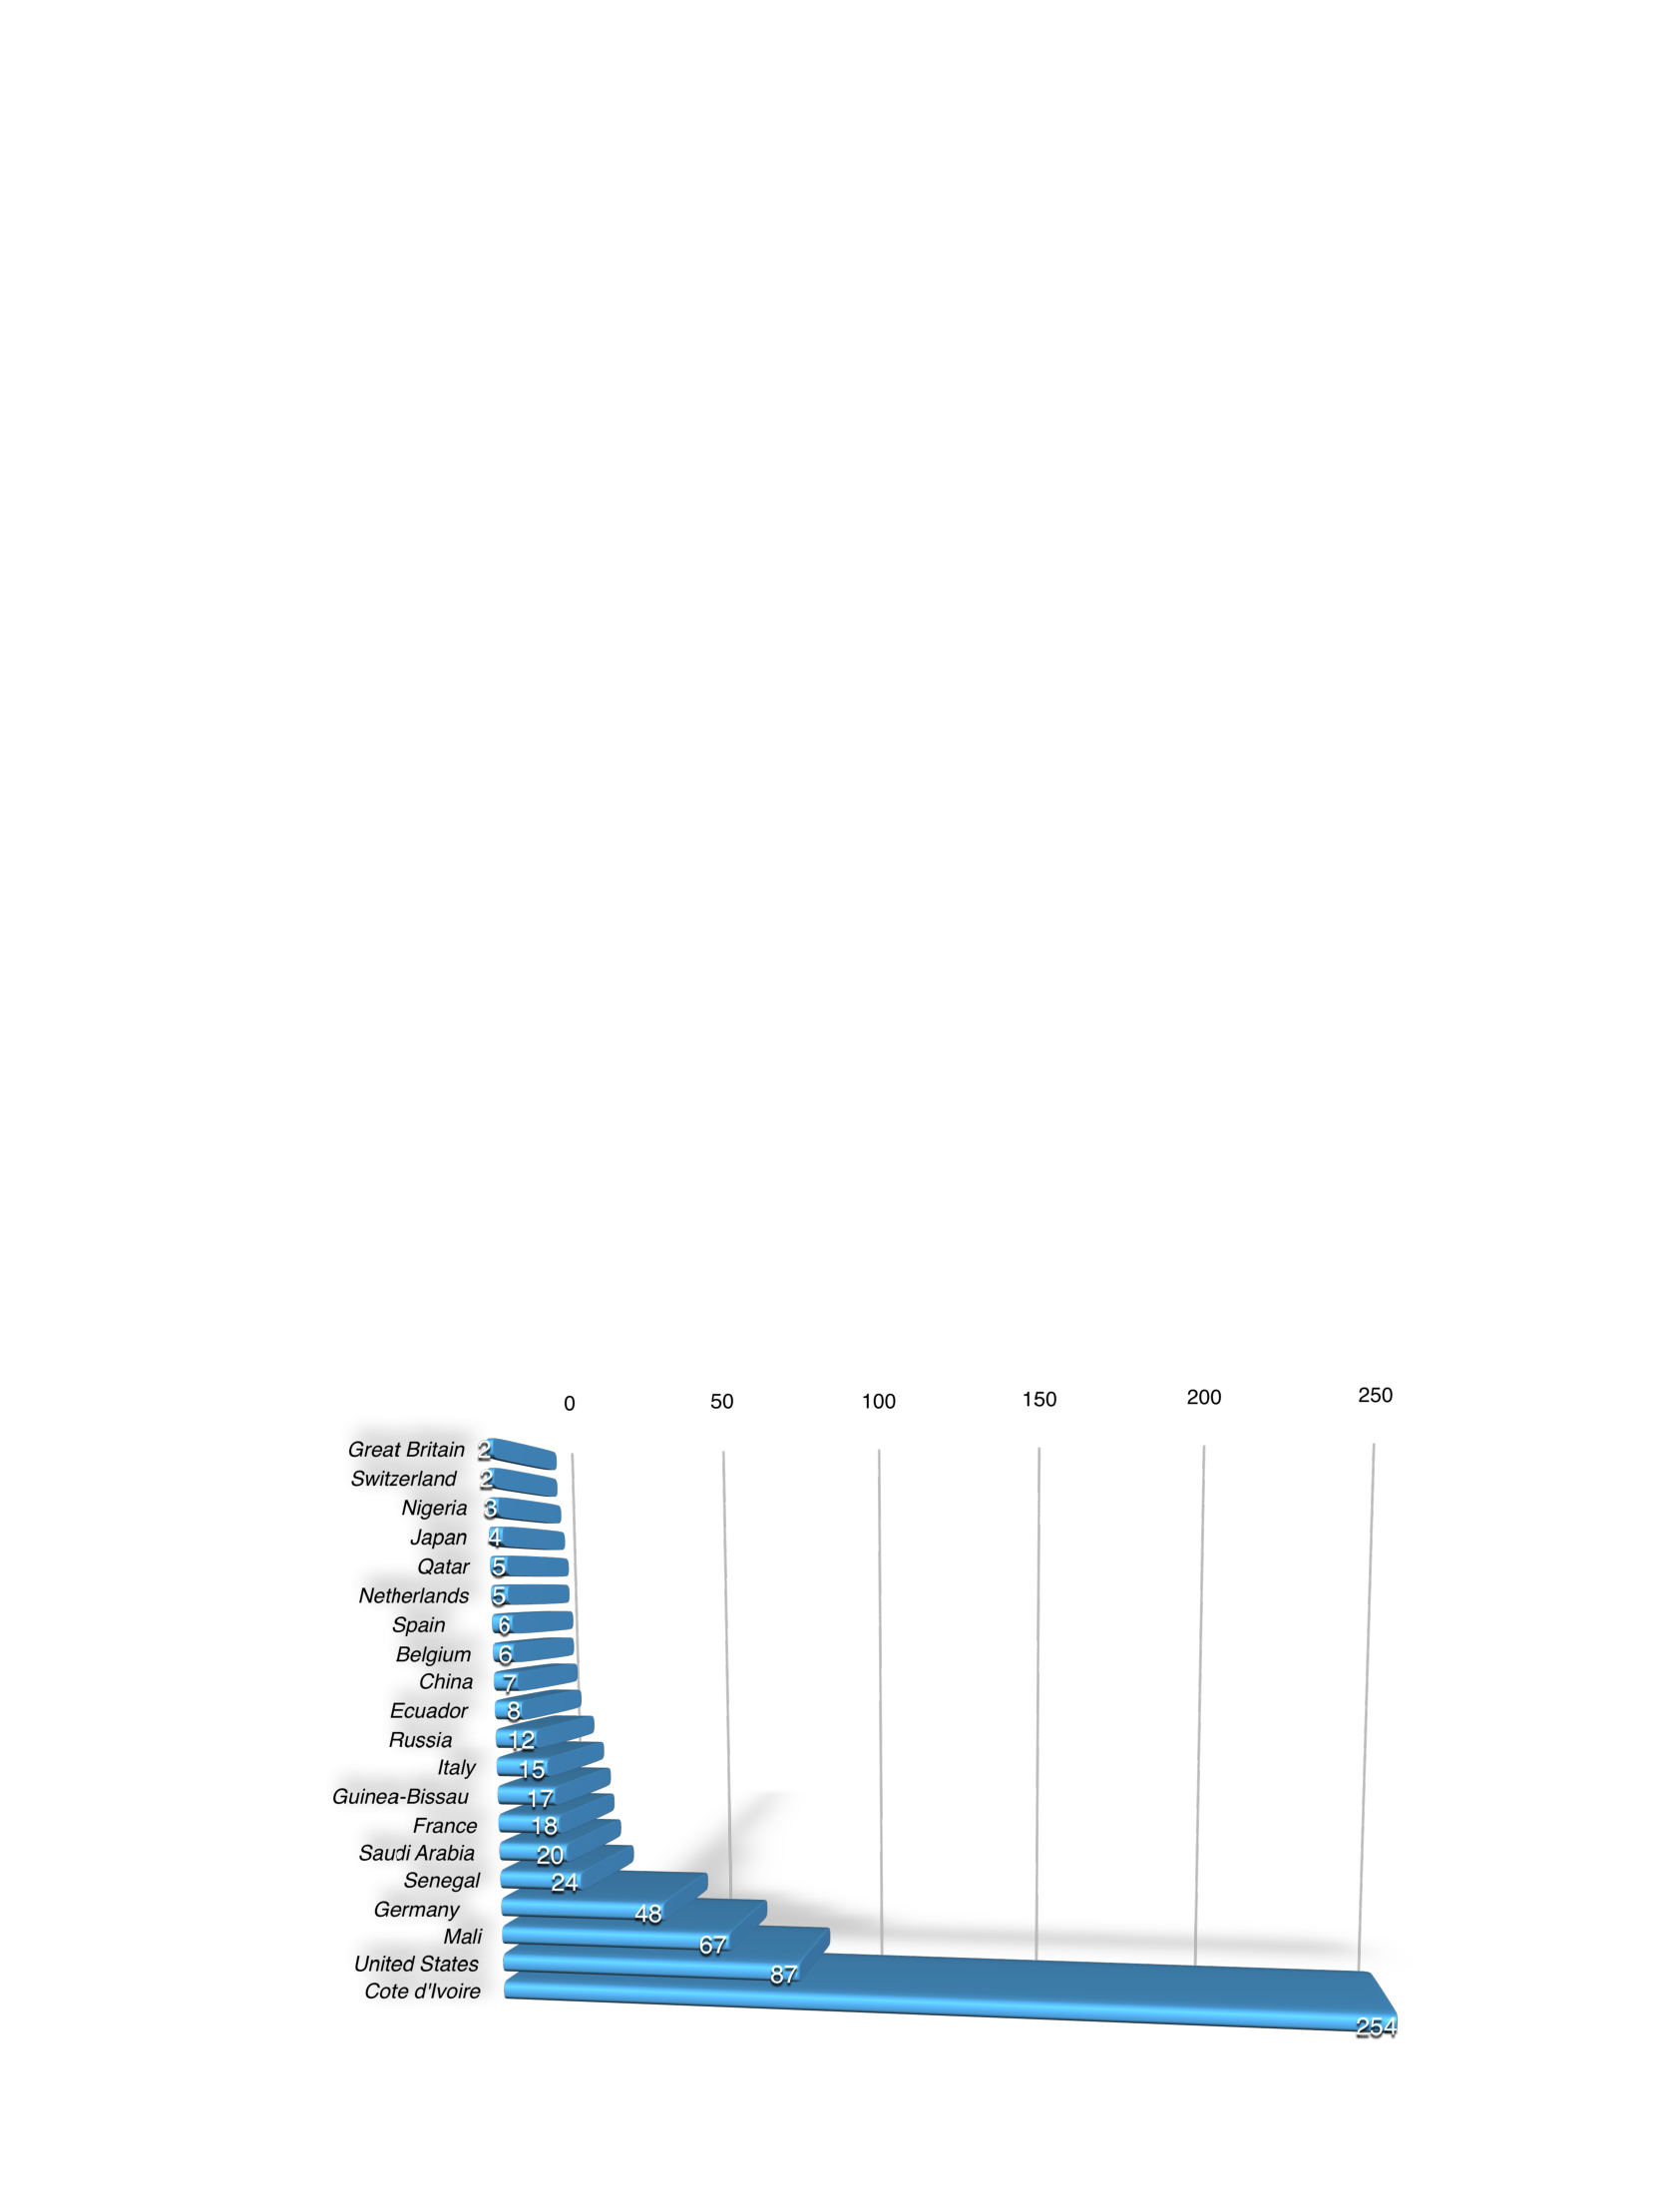
\includegraphics[scale=.6]{countriesInfected.pdf}
\caption{Potential countries that could get infected and potential number of infected by December 31, 2014}
\label{Fig:world_infected}
\end{figure}

In Figure \ref{Fig:world_infected}, we presented the potential number of infected people by December
31, 2014 in countries other than Guinea, Sierra Leone and Liberia based on our world-wide
simulations. The number for Guinea, Sierra Leone and Liberia are similar to the result presented in
Table \ref{Tb:prediction} in Phase 1 as is expected. We note that, the modified trade network data
that we used is a simplistic realization of the very complex human migration pattern and does not
take into account intricacies involving border restriction, enhanced monitoring, religious and
cultural missions etc. Therefore, result obtained from our simulation  will rather represent  an
upper bound on the potential outbreak of the disease. Alternatively, we can interpret the results as
a measure of relative risk of disease spreads in different countries. It is, however, interesting to
see that the result obtained from such simplistic model represents the reality fairly well. So far,
in addition to  Guinea, Sierra Leone and Liberia, Ebola has spread to Mali, Senegal, Nigeria, United
States and Spain. Our simulation result identified all of these countries successfully. In our
simulation, Cote d'Ivoire is identified as the country with the highest risk of spread apart from
Guinea, Sierra Leone and Liberia. However, so far Cote d'Ivoire is Ebola free, even though it shares
border will all of these three infected countries. The reason of Ebola not spreading in Cote
d'Ivoire in not clear. Several speculations e.g. very strict border patrol, trade ban etc. are
credited in the media. Our simulation result indicated 3 people to be infected in Nigeria, whereas
20 peoples got infected in reality. The reason behind such small number is the lack of sufficient
trades as well as no shared border between Guinea, Sierra Leone, Liberia and Nigeria. So far Lagos
region of Nigeria has been affected the most by Ebola. The airport located in the Lagos region is
the busiest hub in West Africa. It is possible that migration through Lagos airport may be related
to the spread of disease in that region, which is not captured in our model.




\section{Conclusion} In this project, we analyzed 2014 Ebola epidemic in West Africa using
epidemiological and network theories. We divided our work in three phases. In phase 1, we analyzed
the data sets of number of Ebola infected individuals to fit  SEIR model for Guinea, Sierra Leone,
Liberia as well as the West African region. We then used these models to perform short-term
prediction of temporal progression of Ebola epidemic in  Guinea, Sierra Leone, Liberia. In phase 2
of our project, we analyzed the spread of disease in four large scale networks - preferential
attachment network, real world social network, small world network and random network with the aid
of Percolation Theory. In addition to that, we created a very large scale world-wide contact network
and attempt to see the progression of disease among different countries from a single infected
initial node in Guinea. In phase 3 of our project, we created a world-wide human migration network
using a combination of economic trade data and country border information. We then combined this
migration network with the SEIR models from phase 1. We then run the combined network to watch the
temporal progression of disease over the course of one year using a single initial infection in
Guinea and provided short-term prediction of world-wide outbreak of Ebola. Our simulation results
match the real world data fairly well.


%%%%%%%%%%%%%%%%%%%%%%%%%%%%%%%%%%%%%%%%%%%%%%%%%%%%%%%%%%%%

\bibliographystyle{plainnat}
\bibliography{bib_ref}



%%%%%%%%%%%%%%%%%%%%%%%%%%%%%%%%%%%%%%%%%%%%%%%%%%%%%%%%%%%%

\begin{appendix}


\begin{table}[h]

\caption{Parameter estimation for Ebola SEIR model (Guinea \& Sierra Leone)}
%\hrule
\centering
\tiny
\parbox{.55\linewidth}{\centering
\ra{1.3}
\begin{tabular}{@{}crccc@{}}%\toprule
& \multicolumn{3}{c}{\textbf{Guinea}} &  \\
\cmidrule{2-4}
\textbf{Incidence Dependent Parameters} & \textit{Value} && \textit{Comments} \\
\midrule
Initial Case $t_0$ & December 2, 2013 &  & one person fell ill\\
$S_0$ & 0& & -\\
$E_0$ & 0& & -\\
$I_0$ & 1& & -\\
$R_0$ & 0& & -\\
$C_0$ & 1& &-\\
Intervention time & March 2, 2014 &  & Gov. of Guinea informed WHO\\
$\tau$ &110 & & -\\
\cmidrule{2-4}
\textbf{Estimated Parameters} & \textit{Value} & \textit{95\% CI} & \textit{Comments} \\
\midrule
Incubation Time $1/k$ &6.3 & - & based on previous works\\
Infection Time $1/\gamma$ &5.4957 & [5.43, 5.545] & -\\
$\beta_0$ &0.2407 & [0.2374, 0.244] & -\\
$\beta_1$ &0.2084 & [0.2033, 0.2135] & -\\
$q$ &32 & [0.1, 100] & -\\
Fatality Rate &0.67 & - & -\\
$R_0$ &1.323 &[1.295, 1.341] &-\\
$R_1$ &1.145 & - &-\\
\end{tabular}
}
%\end{table*}
\parbox{.3\linewidth}{
%\begin{table*}
\centering
\ra{1.3}
\begin{tabular}{@{}crccc@{}}%\toprule
\multicolumn{3}{c}{\textbf{Sierra Leone}} &  \\
\cmidrule{1-3}
%\multicolumn{3}{c}{ {Incidence Dependent Parameters}} &  \\
%\midrule
\textit{Value} && \textit{Comments} \\
\cmidrule{1-3}
April 23, 2014 &  & one person fell ill \cite{}\\
0& & -\\
0& & -\\
1& & -\\
0& & -\\
1& &-\\
June 12, 2014 &  & Country declared emergency\\
50 & & -\\
%\midrule
%\multicolumn{3}{c}{ {Estimated Parameters}} &  \\
\cmidrule{1-3}
\textit{Value} & \textit{95\% CI} & \textit{Comments} \\
\midrule
6.3 & - & based on previous works\\
6.386 & [6.2112, 6.4733] & -\\
0.356 & [0.3391, 0.3643] & -\\
0.195 & [0.1926, 0.1988] & -\\
0.47 & [0.1, 7.07] & -\\
0.289 & - & -\\
2.27 & - &-\\
1.24 & - &-\\
%\bottomrule
\end{tabular}
%\caption{Caption}
}
%\bottomrule
\label{Table:parameter}
\end{table}

%%%%%%%%%%%%

\begin{table}[h]
\caption{Parameter estimation for Ebola SEIR model (Liberia \& West Africa overall)}
\centering
\tiny
\parbox{.55\linewidth}
{\centering
\ra{1.3}
\begin{tabular}{@{}crccc@{}}%\toprule
& \multicolumn{3}{c}{\textbf{Liberia}} &  \\
%\toprule Liberia Liberia
%& \multicolumn{3}{c}{ {Incidence Dependent Parameters}} &  \\
\cmidrule{2-4}
\textbf{Incidenced Dependent Parameters} & \textit{Value} && \textit{Comments} \\
\midrule
Initial Case $t_0$ & March 31, 2014 &  & official confirmation two infected \cite{}\\
$S_0$ & 0& & -\\
$E_0$ & 0& & -\\
$I_0$ & 2& & -\\
$R_0$ & 0& & -\\
$C_0$ & 2& &-\\
Intervention time & July 30, 2014 &  & School shutdown\\
$\tau$ &120 & & -\\
\midrule
%& \multicolumn{3}{c}{ {Estimated Parameters}} &  \\
%\midrule
\textbf{Estimated Parameters} & \textit{Value} & \textit{95\% CI} & \textit{Comments} \\
\midrule
Incubation Time $1/k$ &6.3 & - & based on previous works \cite{}\\
Infection Time $1/\gamma$ &10.5 & [8.32,10.7] & -\\
$\beta_0$ &0.1697 & [0.167, 0.199] & -\\
$\beta_1$ &0.0001 & [0.0001, 0.097] & -\\
$q$ &0.0068 & [0.0059-0.0187] & -\\
Fatality Rate &0.575 & - & -\\
$R_0$ &1.78 &- &-\\
$R_1$ &0.001 & - &-\\
%\bottomrule
\end{tabular}
}
\parbox{.3\linewidth}
{\centering
\ra{1.3}
\begin{tabular}{@{}crccc@{}}%\toprule
\multicolumn{3}{c}{\textbf{West Africa}} &  \\
\cmidrule{1-3}
%& \multicolumn{3}{c}{ {Incidence Dependent Parameters}} &  \\
%\midrule
 \textit{Value} && \textit{Comments} \\
\midrule
December 2, 2013 &  & one person fell ill in Guinea\\
 0& & -\\
 0& & -\\
 1& & -\\
 0& & -\\
 1& &-\\
 March 2, 2014 &  & Gov. of Guinea informed WHO\\
110 & & -\\
\midrule
%& \multicolumn{3}{c}{ {Estimated Parameters}} &  \\
%\midrule
 \textit{Value} & \textit{95\% CI} & \textit{Comments} \\
\midrule
6.3 & - & based on previous works \cite{}\\
6.8 & - & -\\
0.2 & - & -\\
0 & - & -\\
0 & - & -\\
 & - & -\\
1.36 &- &-\\
- & - &-\\
%\bottomrule
\end{tabular}
}
%\bottomrule
%\hrule
\label{Table:parameter2}
\end{table}

%%%%%%%%%%%%



\subsection*{Contribution from individual team members}
\begin{itemize}
\item{Shafi: } Project idea and research, introduction (Section \ref{sec:Introduction}), literature review (Section \ref{sec:RelatedWork}), country level analysis and prediction using compartmental model (Section \ref{sec:IntraCountry}), world-wide analysis and prediction (Section \ref{sec:Worldwide} - subsection \ref{SubSec:WorldSystem} and \ref{SubSec:WorldResult}). Coding, simulation and plots related to Figures \ref{Fig:figurePrediction}, \ref{Fig:worldtrade}, \ref{Fig:world_infected} and Tables \ref{Tb:prediction}, \ref{Table:parameter}, \ref{Table:parameter2}.

\item{Mike: } Project idea and research, helped with literature review, data processing and generation of inter-country migration numbers (Sections \ref{SubSec:TradeData}, \ref{SubSec:LocalData}), helped with performance optimization, parallelization, and EC2 simulation of intra-country percolation model (Section \ref{sec:NetworkModel}), generation of global networks, implementation and execution of global network-based SEIR simulation (Section \ref{SubSec:GraphX}), proof-reading of report.

\item {Romit: } Project idea and research, introduction (Section \ref{sec:Introduction}), exploring the MCMC approach for compartmental model  and developed code.
Data collection and analysis, coding the two simulation model based on percolation theory and running the simulations on EC2, analyzing results and plotting the graphs and generating prediction numbers (Section \ref{sec:NetworkModel})
Figures \ref{Fig:Network_Transmissibility}, \ref{Fig:Network_MinDegree}
Tables \ref{Tb:Transmissibility}, \ref{Tb:prediction_networkm}
\end{itemize}
\end{appendix}



\end{document}
